\section{Recursive Neural Tensor Network}
In this section, we will first introduce how Recursive Neural Network (RNN) is applies to sentiment and then about the Recursive Neural Tensor Network (RNTN). This section is a summary of "Recursive Deep Models for Semantic Compositionally Over a Sentiment Treebank" (Socher et al,. 2013). 
\subsection{RNN: Recursive Neural Network}
We represent each word as a $d-$dimensional vector. When an $n-$gram is given to the compositional models, it is parsed into a binary tree (as in Figure \ref{trigram}). We compute the parent vector in a bottom up fashion using a compositionally function $g$ and use node vectors as features for a classifier at that node. 
\begin{figure}[H]
\begin{center}
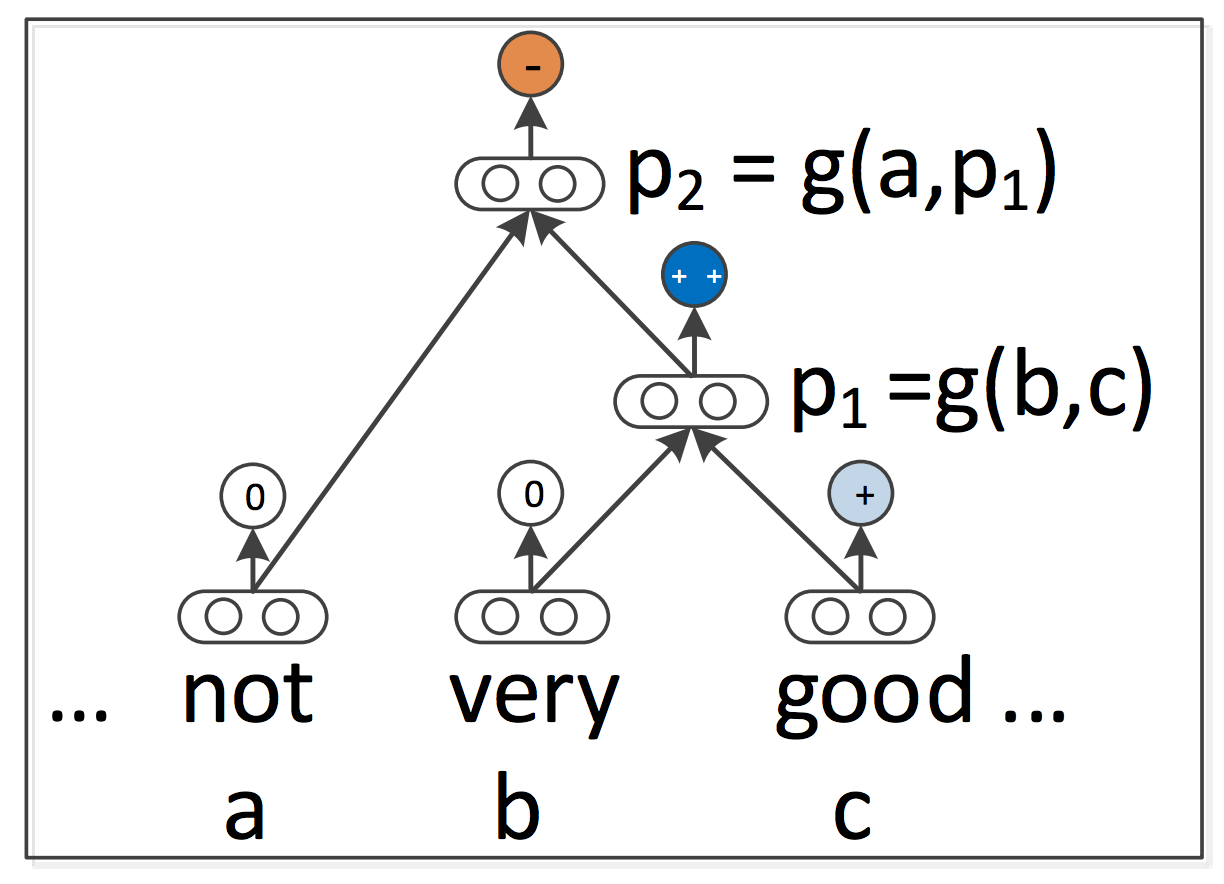
\includegraphics[width = 0.45\textwidth]{pic/trigram.png}
\caption{\label{trigram}Trigram Example}
\end{center}
\end{figure}

RNNs use the following equations to compute the parent vectors: 
\begin{equation*}
p_1 = f \left( W 
\begin{bmatrix}
b \\ c
\end{bmatrix}
 \right), 
p_2 = f \left( W 
\begin{bmatrix}
a \\ p1
\end{bmatrix}
 \right)
\end{equation*}
where $f = \textrm{tanh}$ is standard element-wise nonlinearity. $W \in \mathbb{R}^{d \times 2d}$ is the main parameter to learn. 

\section{RNTN: Recursive Neural Tensor Network}

The main idea behind Recursive Neural Tensor Network(RNTN) is to use the same, tensor based composition function for all node to the reduce the computation complexity. 